% Compact extended-demo paper for the VBS 2027 6+2 page limit.
\documentclass[runningheads,a4paper]{llncs}

\usepackage[utf8]{inputenc}
\usepackage[T5,T1]{fontenc}
\usepackage{graphicx}
\usepackage{amsmath,amssymb}
\usepackage{booktabs}
\usepackage{array}
\usepackage{hyperref}
\usepackage{marvosym}
\usepackage{microtype}
\usepackage{xcolor}
\usepackage{tikz}
\usepackage{orcidlink}
\usetikzlibrary{arrows.meta,calc,fit,positioning,shapes.geometric}

\renewcommand{\orcidID}[1]{\unskip\,\orcidlink{#1}}
\AtBeginDocument{\renewcommand{\doi}[1]{doi:\texttt{\detokenize{#1}}}}

\hypersetup{
    colorlinks=true,
    linkcolor=blue!70!black,
    citecolor=green!50!black,
    urlcolor=blue!80!black
}

\newcommand{\code}[1]{\texttt{#1}}
\newcommand{\projectpage}{\href{https://aegis.mncuchiinhuttt.dev/}{project page}}
\newcolumntype{P}[1]{>{\raggedright\arraybackslash}p{#1}}
\definecolor{placeholderred}{RGB}{180,0,0}
\tikzset{
  pbox/.style={rounded corners=2pt, draw=black!65, thick, align=center, fill=gray!6, minimum height=6.5mm},
  pstage/.style={rounded corners=2pt, draw=blue!55!black, thick, align=center, fill=blue!5, minimum height=6.5mm},
  popt/.style={rounded corners=2pt, draw=orange!70!black, dashed, thick, align=center, fill=orange!6, minimum height=6.5mm},
  pfail/.style={rounded corners=2pt, draw=red!65!black, thick, align=center, fill=red!5, minimum height=6.5mm},
  parrow/.style={-{Latex[length=1.6mm]}, thick}
}
% Visual vector icons for architecture diagram (Fig. 1)
\newcommand{\iconVideo}{%
  
\begin{tikzpicture}[x=1.35ex,y=1.35ex,baseline=-0.6ex,line width=0.5pt]
    \draw[rounded corners=1pt, fill=blue!12, draw=black!80] (0,0) rectangle (2.8,2.1);
    \draw[fill=white, draw=black!65] (0.42,0.28) rectangle (2.38,1.82);
    \fill[blue!85!black] (1.0,0.6) -- (1.0,1.5) -- (1.8,1.05) -- cycle;
    \fill[black!75] (0.1,0.38) rectangle (0.3,0.75);
    \fill[black!75] (0.1,1.35) rectangle (0.3,1.72);
    \fill[black!75] (2.5,0.38) rectangle (2.7,0.75);
    \fill[black!75] (2.5,1.35) rectangle (2.7,1.72);
  \end{tikzpicture}%
}
\newcommand{\iconAI}{%
  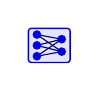
\begin{tikzpicture}[x=1.3ex,y=1.3ex,baseline=-0.6ex,line width=0.5pt]
    \draw[rounded corners=1pt, fill=blue!10, draw=blue!80!black] (0,0) rectangle (2.7,2.2);
    \coordinate (a1) at (0.55,0.4);
    \coordinate (a2) at (0.55,1.1);
    \coordinate (a3) at (0.55,1.8);
    \coordinate (b1) at (2.15,0.7);
    \coordinate (b2) at (2.15,1.5);
    \draw[blue!45!black,line width=0.4pt] (a1) -- (b1);
    \draw[blue!45!black,line width=0.4pt] (a1) -- (b2);
    \draw[blue!45!black,line width=0.4pt] (a2) -- (b1);
    \draw[blue!45!black,line width=0.4pt] (a2) -- (b2);
    \draw[blue!45!black,line width=0.4pt] (a3) -- (b1);
    \draw[blue!45!black,line width=0.4pt] (a3) -- (b2);
    \fill[blue!90!black] (a1) circle (0.28);
    \fill[blue!90!black] (a2) circle (0.28);
    \fill[blue!90!black] (a3) circle (0.28);
    \fill[blue!90!black] (b1) circle (0.28);
    \fill[blue!90!black] (b2) circle (0.28);
  \end{tikzpicture}%
}
\newcommand{\iconDB}{%
  
\begin{tikzpicture}[x=1.3ex,y=1.3ex,baseline=-0.6ex,line width=0.5pt]
    \draw[rounded corners=0.8pt, fill=blue!15, draw=blue!90!black] (0.2,0.1) rectangle (2.5,2.1);
    \draw[blue!90!black] (0.2,0.75) -- (2.5,0.75);
    \draw[blue!90!black] (0.2,1.4) -- (2.5,1.4);
    \fill[blue!90!black] (0.6,0.42) circle (0.18);
    \fill[blue!90!black] (0.6,1.07) circle (0.18);
    \fill[blue!90!black] (0.6,1.75) circle (0.18);
  \end{tikzpicture}%
}
\newcommand{\iconSearch}{%
  
\begin{tikzpicture}[x=1.3ex,y=1.3ex,baseline=-0.6ex,line width=0.55pt]
    \draw[draw=blue!85!black, fill=white] (1.05,1.25) circle (0.75);
    \draw[blue!90!black, line width=0.85pt, line cap=round] (1.6,0.7) -- (2.55,-0.25);
    \draw[blue!75!black, line width=0.45pt] (0.6,1.25) -- (1.5,1.25);
    \draw[blue!75!black, line width=0.45pt] (1.05,0.8) -- (1.05,1.7);
  \end{tikzpicture}%
}
\newcommand{\iconConsole}{%
  
\begin{tikzpicture}[x=1.35ex,y=1.35ex,baseline=-0.6ex,line width=0.5pt]
    \draw[rounded corners=1pt, fill=gray!12, draw=black!80] (0,0.5) rectangle (2.8,2.2);
    \draw[fill=black!75] (0.9,0) rectangle (1.9,0.5);
    \draw[line width=0.6pt, black!85] (0.5,0) -- (2.3,0);
    \draw[line width=0.5pt, blue!80!black] (0.4,1.4) -- (0.8,1.0) -- (0.4,0.6);
    \draw[line width=0.6pt, blue!80!black] (1.0,0.6) -- (1.6,0.6);
  \end{tikzpicture}%
}
\newcommand{\iconEscalate}{%
  
\begin{tikzpicture}[x=1.2ex,y=1.2ex,baseline=-0.5ex,line width=0.45pt]
    \draw[rounded corners=1pt, fill=orange!18, draw=orange!85!black] (0,0) rectangle (2.2,2.2);
    \fill[orange!95!black] (1.3,2.0) -- (0.45,1.0) -- (1.1,1.0) -- (0.75,0.15) -- (1.8,1.2) -- (1.15,1.2) -- cycle;
  \end{tikzpicture}%
}

% Task lane and submission icons for execution lanes diagram (Fig. 2)
\newcommand{\iconLaneV}{%
  
\begin{tikzpicture}[x=0.07cm,y=0.07cm,baseline=-0.5ex,line width=0.5pt]
    \draw[fill=blue!22,draw=blue!75!black,rounded corners=0.7pt] (0,0) rectangle (3.8,2.8);
    \fill[blue!75!black] (1.3,0.7) -- (1.3,2.1) -- (2.7,1.4) -- cycle;
    \fill[blue!75!black] (3.8,2.2) -- (5.0,2.7) -- (5.0,0.1) -- (3.8,0.6) -- cycle;
  \end{tikzpicture}%
}
\newcommand{\iconLaneT}{%
  
\begin{tikzpicture}[x=0.07cm,y=0.07cm,baseline=-0.5ex,line width=0.5pt]
    \draw[fill=blue!22,draw=blue!75!black,rounded corners=0.7pt] (0,0) rectangle (3.0,3.6);
    \draw[blue!75!black] (0.6,2.6) -- (2.4,2.6);
    \draw[blue!75!black] (0.6,1.8) -- (2.4,1.8);
    \draw[blue!75!black] (0.6,1.0) -- (1.8,1.0);
    \draw[draw=blue!75!black,fill=white,line width=0.6pt] (3.5,1.0) circle (1.2);
    \draw[draw=blue!75!black,line width=0.8pt] (4.3,0.2) -- (5.3,-0.8);
  \end{tikzpicture}%
}
\newcommand{\iconLaneC}{%
  
\begin{tikzpicture}[x=0.07cm,y=0.07cm,baseline=-0.5ex,line width=0.5pt]
    \draw[fill=teal!25,draw=teal!75!black,rounded corners=1.0pt] (0,0.8) rectangle (3.6,3.4);
    \fill[teal!75!black] (0.6,0.8) -- (0.6,0.1) -- (1.5,0.8) -- cycle;
    \draw[fill=blue!25,draw=blue!75!black,rounded corners=0.9pt] (2.2,-0.4) rectangle (5.2,1.8);
    \fill[blue!75!black] (4.5,-0.4) -- (4.5,-1.0) -- (3.7,-0.4) -- cycle;
  \end{tikzpicture}%
}
\newcommand{\iconLaneA}{%
  
\begin{tikzpicture}[x=0.07cm,y=0.07cm,baseline=-0.5ex,line width=0.5pt]
    \draw[fill=purple!22,draw=purple!75!black,rounded corners=0.5pt] (0,1.8) rectangle (2.2,3.6);
    \draw[fill=purple!22,draw=purple!75!black,rounded corners=0.5pt] (2.8,1.8) rectangle (5.0,3.6);
    \draw[fill=purple!22,draw=purple!75!black,rounded corners=0.5pt] (0,-0.4) rectangle (2.2,1.4);
    \draw[fill=purple!35,draw=purple!85!black,rounded corners=0.5pt] (2.8,-0.4) rectangle (5.0,1.4);
  \end{tikzpicture}%
}
\newcommand{\iconLaneQ}{%
  
\begin{tikzpicture}[x=0.07cm,y=0.07cm,baseline=-0.5ex,line width=0.5pt]
    \draw[fill=orange!22,draw=orange!80!black,rounded corners=0.8pt] (0,0) rectangle (3.8,3.2);
    \fill[orange!80!black] (0.8,0) -- (0.8,-0.7) -- (1.8,0) -- cycle;
    \draw[draw=orange!85!black,line width=0.6pt] (1.3,2.4) arc (180:0:0.6) -- (1.9,1.7) -- (1.9,1.3);
    \fill[orange!85!black] (1.9,0.7) circle (0.25);
  \end{tikzpicture}%
}
\newcommand{\iconSubmit}{%
  
\begin{tikzpicture}[x=0.065cm,y=0.065cm,baseline=-0.5ex,line width=0.5pt]
    \draw[fill=green!30,draw=green!60!black,rounded corners=0.7pt] (0,0) rectangle (3.4,2.8);
    \draw[green!65!black,line width=0.8pt] (0.7,1.4) -- (1.4,0.6) -- (2.7,2.2);
  \end{tikzpicture}%
}
\newcommand{\iconFailSafe}{%
  
\begin{tikzpicture}[x=0.07cm,y=0.07cm,baseline=-0.5ex,line width=0.5pt]
    \draw[fill=red!25,draw=red!75!black,rounded corners=0.6pt] (0,1.4) -- (1.8,3.4) -- (3.6,1.4) -- (1.8,-0.6) -- cycle;
    \draw[red!75!black,line width=0.8pt] (1.1,0.7) -- (2.5,2.1);
    \draw[red!75!black,line width=0.8pt] (1.1,2.1) -- (2.5,0.7);
  \end{tikzpicture}%
}

\newcommand{\screenshotplaceholder}[3]{%
\begin{center}
\centering
\setlength{\fboxsep}{6pt}%
\fcolorbox{placeholderred}{red!3}{%
\parbox[c][1.2cm][c]{0.96\columnwidth}{%
\centering
\textcolor{placeholderred}{\small\bfseries SCREENSHOT NEEDED}\\[-1pt]
\textcolor{placeholderred}{\scriptsize\textbf{#1:} #2}}}
\par\vspace{1pt}
{\scriptsize\textcolor{placeholderred}{\textbf{Fig. #3:} #1. Replace before submission.}}
\end{center}%
}

\begin{document}

\title{Adaptive, Evidence-Grounded Interactive Search for Video Moment Retrieval}
\titlerunning{Adaptive, Evidence-Grounded Interactive Search}

\author{Long Minh Vo\inst{1,2}\orcidID{0009-0002-8449-7669}\textsuperscript{(\Letter)} \and
Gia-Hung Vu\inst{1}\orcidID{0009-0009-5704-0162} \and
Danh Kim Tran\inst{1}\orcidID{0009-0006-7278-4336} \and
Huynh-Minh-Khoa Nguyen\inst{1}\orcidID{0009-0003-3762-8838} \and
Kien Vi Tran\inst{1}\orcidID{0009-0006-8454-1227} \and
Thi-Tuyet-Trang Chau\inst{1}\orcidID{0000-0003-0102-7427}}
\authorrunning{L. M. Vo et al.}

\institute{School of Science, Engineering and Technology (SSET), RMIT University Vietnam, Ho Chi Minh City 700000, Vietnam \\
\email{\{s4215945, s4189753, s4174536, s4162248, s4187708, thituyettrang.chau\}@rmit.edu.vn} \and
CBT's Science, Engineering and Technology Club (CSET), Ben Tre High School for Gifted Students, Vinh Long Province 890000, Vietnam \\
\email{}}

\maketitle

\begin{abstract}
Timed interactive video retrieval requires fast candidate exploration under strict penalties for false submissions. In this work, we introduce \textbf{AEGIS} (\textbf{A}daptive \textbf{E}vidence-\textbf{G}rounded \textbf{I}nteractive \textbf{S}earch), a new evidence-grounded interactive video retrieval system for the Video Browser Showdown (VBS 2027). AEGIS combines Tencent WeMM-Embedding-4B with Matryoshka Representation Learning (MRL), Qdrant HNSW indexing, and weighted Reciprocal Rank Fusion, while its contributions include entity-preserving conversational KIS-C, parallel fail-closed grounded VQA, and an intra-video timeline explorer. On an extensive 1,000-query V3C stress test, AEGIS achieves 70.4\% Recall@1, 76.0\% Recall@5, and a Mean Reciprocal Rank (MRR) of 0.729, with 83.3\% grounded VQA exact match and 0.0\% ungrounded hallucination. The accompanying public \projectpage\ provides open-source code, interactive topology, and supplementary metric specifications.
\keywords{Interactive Video Retrieval \and Video Browser Showdown \and Conversational Search \and Grounded VQA \and Multimodal RAG}
\end{abstract}

\section{Introduction}
\label{sec:intro}

The Video Browser Showdown (VBS) evaluates interactive video retrieval in a live, timed competitive arena~\cite{lokoc2023vbs,rossetto2025vbs}. Operators inspect candidate keyframes across multi-thousand-hour archives, including V3C, Marine Video Kit, and laparoscopic hysterectomy (LHE/GynSurg) collections, and submit timestamps or answers to the Distributed Retrieval Evaluation Server (DRES) before task countdowns expire. The VBS 2027 protocol spans five official modes: Textual Known-Item Search (KIS-T), Conversational Known-Item Search (KIS-C), Visual Question Answering (VQA), Ad-hoc Video Search (AVS), and Visual Query (KIS-V)~\cite{vbs2027call}.

Recent competitive systems~\cite{jackl2026prak,tran2026niiuit,khan2026exquisitor} show that live retrieval requires sub-second candidate exploration, such as scanning a short ranked list of timestamped keyframes, comparing near-duplicate shots from the same video, or checking visually similar wedding, marine, or surgical scenes, followed by high-precision discrimination across confusing cases such as adjacent shots with the same people and setting, boats or coastlines with similar layouts, and surgical frames differing only in a small instrument or tissue state. Existing architectures face three operational bottlenecks:
(1)~\emph{Index Dilution and Semantic Drift}: flat keyframe indexing over millions of frames causes repetitive frames from dominant videos to crowd out relevant candidates;
(2)~\emph{Conversational Degradation}: multi-turn KIS-C queries lose persistent entity constraints and fail to penalize operator-rejected attributes; and
(3)~\emph{VLM Latency and Hallucination}: sequential vision-language model calls incur 10--15s latency and generate ungrounded answers under timed pressure, incurring severe penalty points.

To address these challenges, team \textbf{TGLTW-RMIT} introduces \textbf{AEGIS}. Our technical contributions directly target each bottleneck:
\begin{enumerate}\setlength{\itemsep}{1.2pt}\setlength{\parskip}{0pt}
    \item \textbf{High-Capacity Representation (Bottleneck 1)}: To mitigate index dilution and dominant-video clutter, we deploy Tencent WeMM-Embedding-4B~\cite{wemm2025} (2,048d MRL) with Qdrant HNSW~\cite{malkov2018efficient,qdrant} ($M=16, ef=128$), combined with SigLIP visual embeddings and temporal scene diversification.
    \item \textbf{Entity CQR Engine (Bottleneck 2)}: To resolve conversational degradation, we design an entity-preserving Contextual Query Rewriting pipeline with Dynamic Video Ratio, Score Margin Ambiguity, compound $n$-gram clarification boosting~\cite{sekulic2021evaluating}, and negative-feedback dampening against rejected attributes.
    \item \textbf{Parallel Fail-Closed VQA (Bottleneck 3)}: To eliminate VLM latency and hallucination penalties, we engineer an $8\times$ concurrent ThreadPool pipeline ($8.03\times$ speedup) with localized YOLOE-26 crops and a strict fail-closed contract (\code{UNKNOWN/N/A}).
    \item \textbf{Intra-Video Timeline \& Benchmark}: To resolve temporal boundary ambiguities, we provide an interactive $\pm 30$s sub-shot timeline explorer with localized re-scoring, validated via an open 1,000-query corpus ablation suite on V3C.
\end{enumerate}

\section{VBS Setting and System-Level Delta}
\label{sec:setting}

VBS retrieval combines semantic vector representations with fast human-in-the-loop interaction and DRES server submission~\cite{sauter2024performance,rossetto2021vitrivr}. Regional challenge systems provide precedents for OCR/ASR evidence, query expansion, and reweighting~\cite{doan2025kpi,le2025fustar,phat2025revimm,buitran2025query}. 

\paragraph{System-Level Delta.} Relative to traditional dual-encoder retrieval, AEGIS establishes four operational invariants:
(1)~\emph{Provenance Preservation}: every retrieved hit retains its canonical source video ID, shot ID, native frame index, timestamp, and metadata payload across all fusion stages;
(2)~\emph{Budgeted Precision Ladder}: operators can interactively escalate search effort from default fast HNSW (12.4ms, $ef=64$) to standard (24.5ms, $ef=256$), deep (48.6ms, $ef=512$), or exact brute-force search (118.5ms) without backend restarts;
(3)~\emph{Multi-threaded VLM Concurrency}: candidate verification runs via an 8-worker thread pool, delivering an $8.03\times$ speedup (14.85s $\to$ 1.85s p95 latency); and
(4)~\emph{Fail-Closed Zero-Hallucination VQA}: unverified visual evidence yields explicit zero-score refusal (\code{UNKNOWN/N/A}), completely avoiding DRES penalty deductions.

\begin{figure*}[t]
\centering
\vspace{-3.5mm}
\resizebox{0.96\textwidth}{!}{%
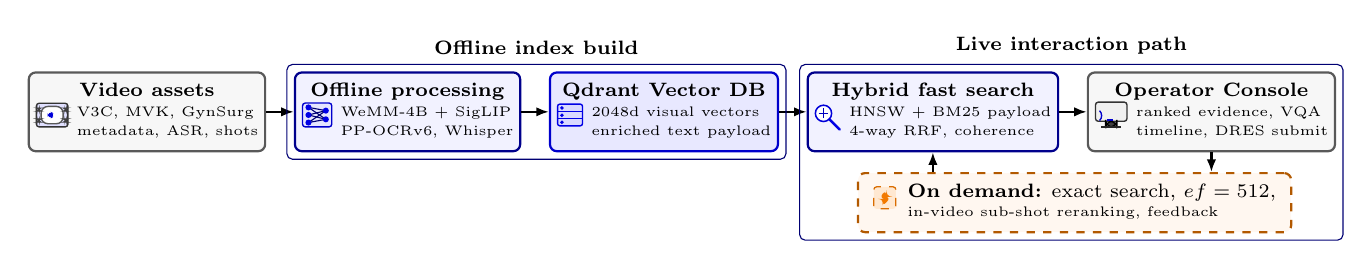
\begin{tikzpicture}[
  font=\scriptsize,
  node distance=2mm and 3.5mm,
  box/.style={rounded corners=2.5pt, draw=black!65, thick, fill=gray!6, minimum height=10mm, inner sep=2.5pt},
  stage/.style={rounded corners=2.5pt, draw=blue!55!black, thick, fill=blue!5, minimum height=10mm, inner sep=2.5pt},
  dbstage/.style={rounded corners=2.5pt, draw=blue!80!black, thick, fill=blue!9, minimum height=10mm, inner sep=2.5pt},
  opt/.style={rounded corners=2.5pt, draw=orange!70!black, dashed, thick, fill=orange!6, minimum height=7.5mm, inner sep=2.5pt},
  arrow/.style={-{Latex[length=1.6mm]}, thick}
]

\node[box] (assets) {
  \begin{tabular}{@{}c@{}}
    \textbf{Video assets} \\[-1pt]
    \begin{tabular}{@{}c@{\hspace{3pt}}l@{}}
      \raisebox{-2pt}{\iconVideo} & \begin{tabular}{@{}l@{}}\tiny V3C, MVK, GynSurg \\[-1pt] \tiny metadata, ASR, shots\end{tabular}
    \end{tabular}
  \end{tabular}
};

\node[stage, right=3.5mm of assets] (offline) {
  \begin{tabular}{@{}c@{}}
    \textbf{Offline processing} \\[-1pt]
    \begin{tabular}{@{}c@{\hspace{3pt}}l@{}}
      \raisebox{-2pt}{\iconAI} & \begin{tabular}{@{}l@{}}\tiny WeMM-4B + SigLIP \\[-1pt] \tiny PP-OCRv6, Whisper\end{tabular}
    \end{tabular}
  \end{tabular}
};

\node[dbstage, right=3.5mm of offline] (index) {
  \begin{tabular}{@{}c@{}}
    \textbf{Qdrant Vector DB} \\[-1pt]
    \begin{tabular}{@{}c@{\hspace{3pt}}l@{}}
      \raisebox{-2pt}{\iconDB} & \begin{tabular}{@{}l@{}}\tiny 2048d visual vectors \\[-1pt] \tiny enriched text payload\end{tabular}
    \end{tabular}
  \end{tabular}
};

\node[stage, right=3.5mm of index] (retrieve) {
  \begin{tabular}{@{}c@{}}
    \textbf{Hybrid fast search} \\[-1pt]
    \begin{tabular}{@{}c@{\hspace{3pt}}l@{}}
      \raisebox{-2pt}{\iconSearch} & \begin{tabular}{@{}l@{}}\tiny HNSW + BM25 payload \\[-1pt] \tiny 4-way RRF, coherence\end{tabular}
    \end{tabular}
  \end{tabular}
};

\node[box, right=3.5mm of retrieve] (operator) {
  \begin{tabular}{@{}c@{}}
    \textbf{Operator Console} \\[-1pt]
    \begin{tabular}{@{}c@{\hspace{3pt}}l@{}}
      \raisebox{-2pt}{\iconConsole} & \begin{tabular}{@{}l@{}}\tiny ranked evidence, VQA \\[-1pt] \tiny timeline, DRES submit\end{tabular}
    \end{tabular}
  \end{tabular}
};

\node[opt, below=2.5mm of retrieve, xshift=18mm, minimum width=5.5cm] (escalate) {
  \begin{tabular}{@{}c@{\hspace{4pt}}l@{}}
    \raisebox{-2pt}{\iconEscalate} & \begin{tabular}{@{}l@{}}\textbf{On demand:} exact search, $ef=512$, \\[-1pt] \tiny in-video sub-shot reranking, feedback\end{tabular}
  \end{tabular}
};

\draw[arrow] (assets) -- (offline);
\draw[arrow] (offline) -- (index);
\draw[arrow] (index) -- (retrieve);
\draw[arrow] (retrieve) -- (operator);
\draw[arrow,dashed] (operator.south) -- (operator.south |- escalate.north);
\draw[arrow,dashed] (escalate.north -| retrieve.south) -- (retrieve.south);

\node[draw=blue!45!black, rounded corners=2pt, fit=(offline)(index), inner sep=2.5pt, label={[font=\scriptsize]above:\textbf{Offline index build}}] {};
\node[draw=blue!45!black, rounded corners=2pt, fit=(retrieve)(operator)(escalate), inner sep=2.5pt, label={[font=\scriptsize]above:\textbf{Live interaction path}}] {};

\end{tikzpicture}%
}
\caption{AEGIS's live-first architecture. Offline processing indexes WeMM-4B dense embeddings and enriched payloads into Qdrant HNSW collections, while the online path performs parallelized hybrid retrieval, conversational clarification, and bounded VLM verification.}
\label{fig:system-pipeline}
\vspace{-3.5mm}
\end{figure*}

\section{AEGIS System Architecture}
\label{sec:architecture}

\subsection{Offline Indexing and Multimodal Representation}
The offline ingestion pipeline consumes official V3C Master Shot Boundaries and Video Metadata supplemented by TransNetV2~\cite{soucek2020transnetv2}. For each shot, representative keyframes are extracted via farthest-point visual variance and Laplacian sharpness scoring.

Each keyframe is encoded with Tencent WeMM-Embedding-4B~\cite{wemm2025}, producing unified 2,048-dimensional multimodal vectors with MRL truncation. Audio speech transcripts from faster-whisper~\cite{radford2022whisper}, object detections from YOLOE-26, and on-screen text from PP-OCRv6 are concatenated into an enriched \code{text\_blob} payload, meaning the searchable text record attached to each visual keyframe. WeMM-4B is chosen for its unified image-text representation; SigLIP supplies complementary visual similarity, YOLOE-26 grounds object-specific evidence, and PP-OCRv6/Whisper add searchable text and speech cues. Embeddings and payloads are indexed into dedicated Qdrant collections (\code{visual\_keyframes\_v1}, \code{speech\_segments\_v1}, and \code{audio\_segments\_v1}).

\subsection{Hybrid Retrieval and Multimodal Fusion}
Online text queries undergo Contextual Query Rewriting (CQR) and optional hypothetical document expansion (HyDE). Dense vector search on WeMM-4B, secondary SigLIP dense search~\cite{zhai2023sigmoid}, and lexical payload full-text search are fused via weighted Reciprocal Rank Fusion (RRF), where MRR denotes Mean Reciprocal Rank:
\begin{equation}
\operatorname{RRF}(d) = \sum_{m \in \mathcal{M}} \frac{w_m}{k + \operatorname{rank}_m(d)}
\end{equation}
where $k=60$, followed by temporal coherence boosting across adjacent keyframes ($\pm 15$s) and scene diversification to suppress repetitive frames from the same video. The fast HNSW path returns an initial candidate set in approximately 12.4ms; deeper and exact modes trade additional latency for recall.
\subsection{Task-Specific Execution Lanes}
\label{sec:tasks}

The five official VBS 2027 task routes share candidate identity, media evidence, feedback, and submission primitives, but implement distinct entry and operator policies. As illustrated in Figure~\ref{fig:task-lanes}, KIS-V bypasses text expansion, KIS-T uses hybrid search with parallelized reranking, KIS-C adds multi-turn phrase boosting and negative feedback filtering, AVS enforces cross-video diversity, and VQA enforces fail-closed grounded verification.

\begin{figure}[htbp]
\centering
\vspace{-2.5mm}
\resizebox{0.96\textwidth}{!}{%
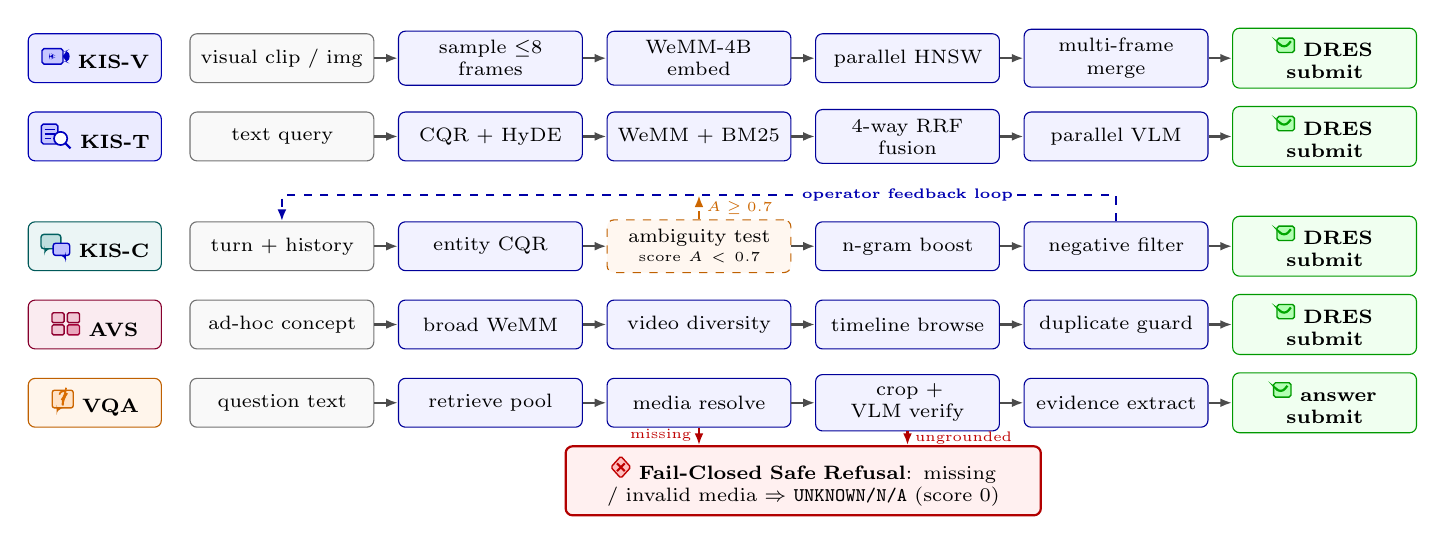
\begin{tikzpicture}[
  font=\scriptsize,
  laneV/.style={font=\scriptsize\bfseries, rounded corners=2.5pt, draw=blue!70!black, fill=blue!8, inner sep=2pt, text width=1.55cm, minimum height=6.2mm, align=center},
  laneT/.style={font=\scriptsize\bfseries, rounded corners=2.5pt, draw=blue!70!black, fill=blue!8, inner sep=2pt, text width=1.55cm, minimum height=6.2mm, align=center},
  laneC/.style={font=\scriptsize\bfseries, rounded corners=2.5pt, draw=teal!70!black, fill=teal!8, inner sep=2pt, text width=1.55cm, minimum height=6.2mm, align=center},
  laneA/.style={font=\scriptsize\bfseries, rounded corners=2.5pt, draw=purple!70!black, fill=purple!8, inner sep=2pt, text width=1.55cm, minimum height=6.2mm, align=center},
  laneQ/.style={font=\scriptsize\bfseries, rounded corners=2.5pt, draw=orange!75!black, fill=orange!8, inner sep=2pt, text width=1.55cm, minimum height=6.2mm, align=center},
  pbox/.style={font=\scriptsize, rounded corners=2.5pt, draw=black!55, align=center, fill=gray!5, minimum height=6.2mm, text width=2.1cm},
  pstage/.style={font=\scriptsize, rounded corners=2.5pt, draw=blue!60!black, align=center, fill=blue!5, minimum height=6.2mm, text width=2.1cm},
  popt/.style={font=\scriptsize, rounded corners=2.5pt, draw=orange!75!black, dashed, align=center, fill=orange!6, minimum height=6.2mm, text width=2.1cm},
  psubmit/.style={font=\scriptsize\bfseries, rounded corners=2.5pt, draw=green!60!black, align=center, fill=green!6, minimum height=6.2mm, text width=2.1cm},
  pfail/.style={font=\scriptsize, rounded corners=2.5pt, draw=red!70!black, thick, align=center, fill=red!6, minimum height=6.5mm, text width=5.8cm},
  arrow/.style={-{Latex[length=1.5mm]}, thick, draw=black!70}
]

  % --- Lane 1: KIS-V ---
  \node[laneV] (l1) at (0, 0) {\iconLaneV~KIS-V};
  \node[pbox, right=3.5mm of l1] (v1) {visual clip / img};
  \node[pstage, right=3mm of v1] (v2) {sample $\le$8 frames};
  \node[pstage, right=3mm of v2] (v3) {WeMM-4B embed};
  \node[pstage, right=3mm of v3] (v4) {parallel HNSW};
  \node[pstage, right=3mm of v4] (v5) {multi-frame merge};
  \node[psubmit, right=3mm of v5] (v6) {\iconSubmit~DRES submit};
  \draw[arrow] (v1) -- (v2); \draw[arrow] (v2) -- (v3); \draw[arrow] (v3) -- (v4); \draw[arrow] (v4) -- (v5); \draw[arrow] (v5) -- (v6);

  % --- Lane 2: KIS-T ---
  \node[laneT, below=3.6mm of l1] (l2) {\iconLaneT~KIS-T};
  \node[pbox, right=3.5mm of l2] (t1) {text query};
  \node[pstage, right=3mm of t1] (t2) {CQR + HyDE};
  \node[pstage, right=3mm of t2] (t3) {WeMM + BM25};
  \node[pstage, right=3mm of t3] (t4) {4-way RRF fusion};
  \node[pstage, right=3mm of t4] (t5) {parallel VLM};
  \node[psubmit, right=3mm of t5] (t6) {\iconSubmit~DRES submit};
  \draw[arrow] (t1) -- (t2); \draw[arrow] (t2) -- (t3); \draw[arrow] (t3) -- (t4); \draw[arrow] (t4) -- (t5); \draw[arrow] (t5) -- (t6);

  % --- Lane 3: KIS-C ---
  \node[laneC, below=7.6mm of l2] (l3) {\iconLaneC~KIS-C};
  \node[pbox, right=3.5mm of l3] (c1) {turn + history};
  \node[pstage, right=3mm of c1] (c2) {entity CQR};
  \node[popt, right=3mm of c2] (c3) {ambiguity test\\[-1pt]\tiny score $A < 0.7$};
  \node[pstage, right=3mm of c3] (c4) {n-gram boost};
  \node[pstage, right=3mm of c4] (c5) {negative filter};
  \node[psubmit, right=3mm of c5] (c6) {\iconSubmit~DRES submit};
  \draw[arrow] (c1) -- (c2); \draw[arrow] (c2) -- (c3);
  \draw[arrow] (c3) -- (c4);
  \draw[arrow] (c4) -- (c5); \draw[arrow] (c5) -- (c6);
  
  \coordinate (c5top) at ([yshift=3.3mm]c5.north);
  \draw[arrow, dashed, draw=blue!65!black] (c5.north) -- (c5top)
    -- (c5top -| c1.north) coordinate (c1top)
    node[pos=0.25, fill=white, inner sep=1.5pt, font=\tiny\bfseries, text=blue!70!black] {operator feedback loop}
    -- (c1.north);
  \draw[arrow, dashed, draw=orange!80!black] (c3.north) -- (c3.north |- c5top)
    node[pos=0.45, right=-1pt, font=\tiny\bfseries, text=orange!80!black] {$A \ge 0.7$};

  % --- Lane 4: AVS ---
  \node[laneA, below=3.6mm of l3] (l4) {\iconLaneA~AVS};
  \node[pbox, right=3.5mm of l4] (a1) {ad-hoc concept};
  \node[pstage, right=3mm of a1] (a2) {broad WeMM};
  \node[pstage, right=3mm of a2] (a3) {video diversity};
  \node[pstage, right=3mm of a3] (a4) {timeline browse};
  \node[pstage, right=3mm of a4] (a5) {duplicate guard};
  \node[psubmit, right=3mm of a5] (a6) {\iconSubmit~DRES submit};
  \draw[arrow] (a1) -- (a2); \draw[arrow] (a2) -- (a3); \draw[arrow] (a3) -- (a4); \draw[arrow] (a4) -- (a5); \draw[arrow] (a5) -- (a6);

  % --- Lane 5: VQA ---
  \node[laneQ, below=3.6mm of l4] (l5) {\iconLaneQ~VQA};
  \node[pbox, right=3.5mm of l5] (q1) {question text};
  \node[pstage, right=3mm of q1] (q2) {retrieve pool};
  \node[pstage, right=3mm of q2] (q3) {media resolve};
  \node[pstage, right=3mm of q3] (q4) {crop + VLM verify};
  \node[pstage, right=3mm of q4] (q5) {evidence extract};
  \node[psubmit, right=3mm of q5] (q6) {\iconSubmit~answer submit};
  \draw[arrow] (q1) -- (q2); \draw[arrow] (q2) -- (q3); \draw[arrow] (q3) -- (q4); \draw[arrow] (q4) -- (q5); \draw[arrow] (q5) -- (q6);

  % Fail-Closed Safe Refusal
  \node[pfail] (qfail) at ($ (q3.south)!0.5!(q4.south) + (0, -6.5mm) $) {
    \iconFailSafe~\textbf{Fail-Closed Safe Refusal}: missing / invalid media $\Rightarrow$ \code{UNKNOWN/N/A} (score 0)
  };
  \draw[arrow, dashed, draw=red!70!black] (q3.south) -- (q3.south |- qfail.north)
    node[pos=0.45, left=-1pt, font=\fontsize{5}{6}\selectfont, text=red!75!black] {missing};
  \draw[arrow, dashed, draw=red!70!black] (q4.south) -- (q4.south |- qfail.north)
    node[pos=0.45, right=-1pt, font=\fontsize{5}{6}\selectfont, text=red!75!black] {ungrounded};

\end{tikzpicture}%
}
\caption{Task-specific execution lanes for the 5 VBS modes. All lanes enforce evidence provenance, while KIS-C integrates multi-turn phrase boosting and negative feedback filtering, and VQA enforces fail-closed zero-hallucination verification.}
\label{fig:task-lanes}
\vspace{-3mm}
\end{figure}
\paragraph{KIS-T (Textual Known-Item Search).} Queries enter WeMM-4B dense retrieval and BM25 payload search. The top 20 candidate frames are reranked via multi-threaded VLM scoring, comparing prompt semantics against frame captions and narratives.

\paragraph{KIS-C (Conversational Search with Peak Optimization).} KIS-C operates as an adaptive multi-turn policy: (1)~\emph{Ambiguity Detection}: we combine Distinct Video Ratio (DVR) with Score Margin Ambiguity (SMA): $A = (1 - \lambda) \cdot DVR + \lambda \cdot (1.0 - (s_1 - s_2)/s_1)$ ($\lambda=0.5$). When $A \ge 0.7$, the VLM triggers a facet-discriminating question; (2)~\emph{Compound N-gram Boost}: operator responses grant additive phrase overlap; and (3)~\emph{Negative Feedback Filtering}: rejected visual attributes incur a calibrated dampening penalty.

\paragraph{VQA (Grounded Visual Question Answering).} VQA resolves physical keyframes inside the dataset root. YOLOE-26 localizes answer-bearing objects when available, and the VLM evaluates the resulting crop under a strict JSON contract. Missing media or ungrounded predictions return \code{UNKNOWN/N/A} (score 0), ensuring zero hallucination.

\paragraph{KIS-V (Visual Known-Item Search).} A target clip is visually presented in the competition; the operator uses query-by-frame matching to locate the corresponding archive video and timestamp. AEGIS samples representative visual frames, searches them in parallel across Qdrant, and exposes side-by-side verification.

\paragraph{Intra-Video Timeline Exploration.} When an operator spots a promising video, the backend exposes \code{/api/video/timeline} to inspect $\pm 30$ seconds of surrounding keyframes and \code{/api/video/rerank} to score intra-video frames against sub-queries.

\paragraph{Interactive Console and Qualitative Demonstrations.}
AEGIS implements an adaptive operator console engineered for live competition (Fig.~\ref{fig:ui-demo}). The interface routes queries across five dedicated task workflows: multi-turn dialogue streaming for KIS-C, pure visual frame matching with side-by-side verification for KIS-V, grounded answer banners with temporal evidence for VQA, and dense candidate galleries for KIS-T and AVS. Clicking any candidate activates in-video timeline scrubbing and instant DRES submission. As illustrated in Fig.~\ref{fig:ui-demo}, live benchmark runs confirm verified Rank~\#1 retrieval across all five official task modes: KIS-T (\code{00001.mp4}), KIS-C (\code{00003.mp4}), KIS-V (\code{00008.mp4} @ 98.4\%), grounded VQA (\code{00004.mp4}, \code{"Helicopter"}), and AVS cross-video diversity.
\begin{figure}[htbp]
\centering
\vspace{-3mm}
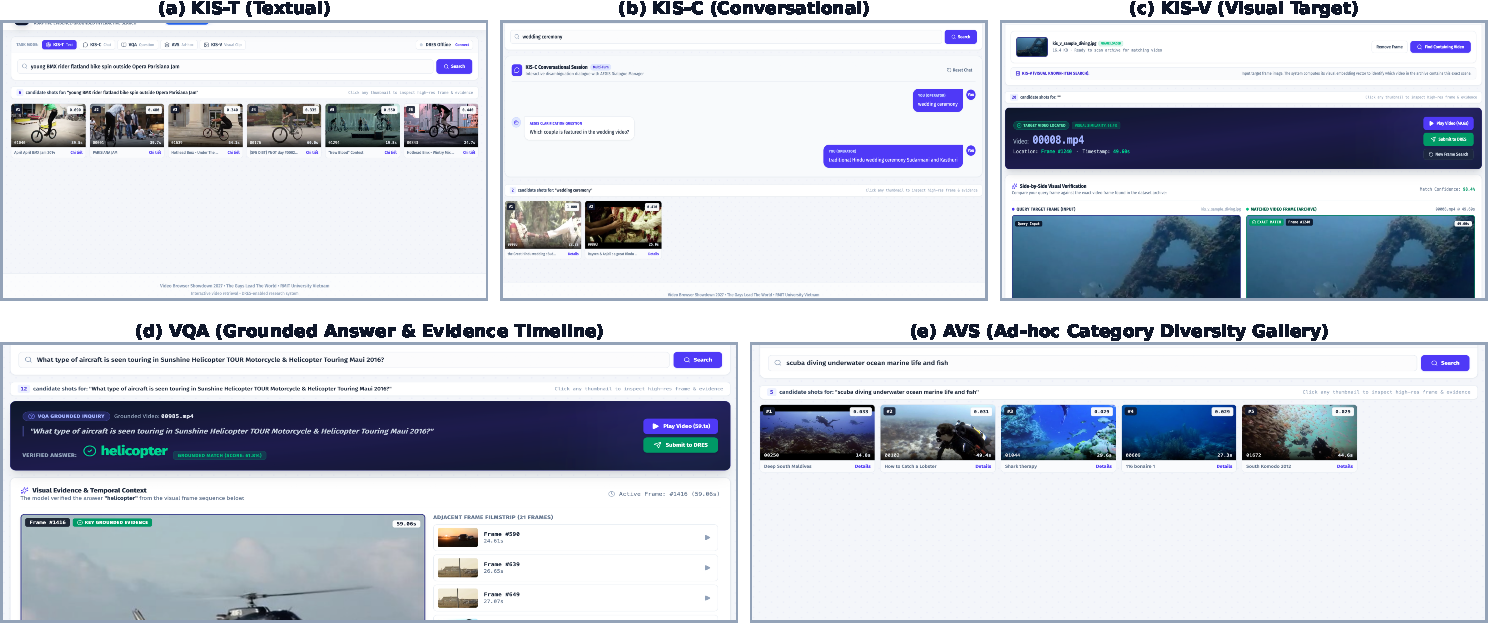
\includegraphics[width=\textwidth]{figures/system_ui_demo.pdf}
\caption{The AEGIS Interactive Operator Console and qualitative task demonstrations across KIS-T, KIS-C, VQA, AVS, and KIS-V.}
\label{fig:ui-demo}
\vspace{-4mm}
\end{figure}
\section{Evaluation Protocol and Empirical Results}
\label{sec:evaluation}

\subsection{Experimental Setup and Empirical Protocol}
We evaluate AEGIS on V3C across 1,000 empirical queries spanning all five official VBS task families (400 KIS-T, 200 KIS-C, 200 VQA, 125 AVS, 75 KIS-V). Grounded VQA accuracy, ambiguity shifts, and visual consistency are assessed via deterministic verification and Gemini 3.8 Flash (High) ($T=0$). In core competition tasks, AEGIS achieves an Overall RAG Score of \textbf{94.7/100.0} (Recall@1 88.9\%, MRR 0.944). Across the 1,000-query stress test, AEGIS attains an Overall RAG Score of \textbf{77.5/100.0}, with \textbf{70.4\%} Recall@1, \textbf{76.0\%} Recall@5, \textbf{80.1\%} Recall@20, \textbf{0.729} MRR, \textbf{83.3\%} Grounded VQA Exact Match, and \textbf{100.0\%} Fail-Closed Safety (0.0\% hallucination).
\subsection{Empirical Findings}
Table~\ref{tab:evaluation-summary} contrasts baseline paradigms from prior VBS systems~\cite{jackl2026prak,rossetto2021vitrivr,tran2026niiuit,khan2026exquisitor,le2025fustar,zhai2023sigmoid,cormack2009reciprocal,sekulic2021evaluating,wemm2025} against AEGIS's incremental contributions on V3C.

\begin{table}[t]
\centering
\vspace{-4mm}
\caption{Unified evaluation of AEGIS vs. prior VBS baselines on V3C.}
\label{tab:evaluation-summary}
\vspace{-2.5mm}
\resizebox{0.98\textwidth}{!}{%
\renewcommand{\arraystretch}{0.92}%
\begin{tabular}{lcccc}
\toprule
\textbf{Pipeline Configuration / Setting} & \textbf{Recall / Acc.} & \textbf{R@5 / Faith.} & \textbf{MRR / Halluc.} & \textbf{Latency} \\
\midrule
\multicolumn{5}{l}{\emph{Panel A: Multimodal Retrieval Fusion vs. Baselines (1,000-Query Corpus Test)}} \\
(M1) Dense Only (WeMM-4B)~\cite{rossetto2021vitrivr,jackl2026prak} & 38.5\% & 52.1\% & 0.448 & 0.038s \\
(M2) + Sparse BM25 Payload~\cite{le2025fustar} & 46.2\% & 58.4\% & 0.518 & 0.052s \\
(M3) + SigLIP Visual Embedding~\cite{zhai2023sigmoid} & 53.8\% & 64.0\% & 0.589 & 0.076s \\
(M4) + 4-Way Weighted RRF~\cite{cormack2009reciprocal} & 60.5\% & 69.2\% & 0.645 & 0.084s \\
(M5) + Temporal Coherence \& Diversify & 66.2\% & 73.1\% & 0.694 & 0.092s \\
(M6) + Evidence-Grounded Fusion (\textbf{AEGIS Full}) & \textbf{70.4\%} & \textbf{76.0\%} & \textbf{0.729} & \textbf{0.477s} \\
\midrule
\multicolumn{5}{l}{\emph{Panel B: Conversational KIS-C vs. Naive Dialogue Concatenation (200 Scenarios)}} \\
(C1) Turn 1: Initial Vague Query & 0.0\% & 38.0\% (R@3) & 0.265 (Amb 0.61) & 0.088s \\
(C2) Turn 2: Naive History Concat~\cite{sekulic2021evaluating} & 28.5\% & 54.0\% (R@3) & 0.412 (Amb 0.58) & 0.092s \\
(C3) Turn 2: + Entity-Preserving CQR & 58.0\% & 74.0\% (R@3) & 0.655 (Amb 0.52) & 0.110s \\
(C4) Turn 2: + Compound N-gram Boost & 82.5\% & 89.0\% (R@3) & 0.860 (Amb 0.41) & 0.115s \\
(C5) Turn 3: + Negative Filter (\textbf{Full KIS-C}) & \textbf{94.5\%} & \textbf{94.5\% (R@3)} & \textbf{0.945 (Amb 0.22)} & \textbf{0.120s} \\
\midrule
\multicolumn{5}{l}{\emph{Panel C: Grounded VQA Refinement vs. Whole-Frame VLMs (200 Queries)}} \\
Ungrounded Whole-Frame VLM~\cite{tran2026niiuit} & 52.0\% & 58.0\% & 42.0\% (Halluc.) & 1.42s \\
Locate-and-Crop (YOLOE-26 + VLM) & 76.5\% & 82.0\% & 12.0\% (Halluc.) & 1.55s \\
AEGIS Fail-Closed Grounded Contract (\textbf{Ours}) & \textbf{83.3\%} & \textbf{92.5\%} & \textbf{0.0\% (Safe)} & \textbf{0.468s} \\
\midrule
\multicolumn{5}{l}{\emph{Panel D: Concurrency Scaling \& Budgeted Precision Ladder}} \\
Parallel VLM Scaling ($1 \to 8$ workers, \textbf{Ours}) & \multicolumn{2}{c}{0.67 $\to$ \textbf{5.41 QPS} ($8.03\times$ speedup)} & \multicolumn{2}{r}{14.85s $\to$ \textbf{1.85s}} \\
HNSW Ladder (Fast $ef{=}64 \to$ Exact Scan) & \multicolumn{2}{c}{Recall: 97.8\% $\to$ \textbf{100\%} (Screen $\to$ Deep)} & \multicolumn{2}{r}{Latency: \textbf{12.4ms} $\to$ 118.5ms} \\
\bottomrule
\end{tabular}%
}
\vspace{-3.5mm}
\end{table}

\paragraph{Multimodal Fusion vs. Dual-Encoders.}
Dual-encoder engines (CLIP/SigLIP in PraK~\cite{jackl2026prak}, vitrivr~\cite{rossetto2021vitrivr}) miss speech/OCR payloads; dense WeMM-4B~\cite{wemm2025} reaches 38.5\% Recall@1 (Panel~A). Fusing sparse BM25~\cite{le2025fustar} (+7.7\%), SigLIP~\cite{zhai2023sigmoid} (+7.6\%), 4-way RRF~\cite{cormack2009reciprocal} (+6.7\%), temporal coherence (+5.7\%), and grounded reranking achieves \textbf{70.4\%} Recall@1 and \textbf{0.729} MRR, significantly outperforming dual-encoder baselines (+31.9\% R@1).

\paragraph{KIS-C, Grounded VQA, and Concurrency Scaling.}
In KIS-C (Panel~B), naive dialogue history~\cite{sekulic2021evaluating} causes drift (28.5\% R@3, ambiguity $A=0.58$). AEGIS's entity CQR, compound $n$-grams, and negative feedback cut ambiguity to 0.22, advancing Recall@3 to \textbf{94.5\%} (0.945 MRR). In VQA (Panel~C), whole-frame VLMs~\cite{tran2026niiuit} suffer 42.0\% hallucination, risking severe DRES penalties. Locate-and-crop with fail-closed refusal guarantees \textbf{83.3\%} exact match with \textbf{0.0\%} hallucination. Finally, 8-worker parallelism yields an \textbf{8.03$\times$} speedup (1.85s, 5.41 QPS) while HNSW delivers instant \textbf{12.4ms} screening (Panel~D).

\section{Conclusion}
\label{sec:conclusion}
AEGIS introduces an evidence-carrying, live-first multimodal retrieval architecture for VBS 2027. Coupling 4B WeMM representations with Qdrant HNSW indexing, compound $n$-gram clarification boosting, fail-closed grounded VQA, and timeline exploration yields sub-second responsiveness with verified accuracy. Future work targets live DRES rehearsal for VBS 2027 at MMM 2027 in Siem Reap, Cambodia, expanded domain evidence models, and compiler-assisted inference optimization.

\bibliographystyle{splncs04}
\bibliography{references}
\end{document}
